% Options for packages loaded elsewhere
\PassOptionsToPackage{unicode}{hyperref}
\PassOptionsToPackage{hyphens}{url}
%
\documentclass[
]{article}
\usepackage{amsmath,amssymb}
\usepackage{lmodern}
\usepackage{ifxetex,ifluatex}
\ifnum 0\ifxetex 1\fi\ifluatex 1\fi=0 % if pdftex
  \usepackage[T1]{fontenc}
  \usepackage[utf8]{inputenc}
  \usepackage{textcomp} % provide euro and other symbols
\else % if luatex or xetex
  \usepackage{unicode-math}
  \defaultfontfeatures{Scale=MatchLowercase}
  \defaultfontfeatures[\rmfamily]{Ligatures=TeX,Scale=1}
\fi
% Use upquote if available, for straight quotes in verbatim environments
\IfFileExists{upquote.sty}{\usepackage{upquote}}{}
\IfFileExists{microtype.sty}{% use microtype if available
  \usepackage[]{microtype}
  \UseMicrotypeSet[protrusion]{basicmath} % disable protrusion for tt fonts
}{}
\makeatletter
\@ifundefined{KOMAClassName}{% if non-KOMA class
  \IfFileExists{parskip.sty}{%
    \usepackage{parskip}
  }{% else
    \setlength{\parindent}{0pt}
    \setlength{\parskip}{6pt plus 2pt minus 1pt}}
}{% if KOMA class
  \KOMAoptions{parskip=half}}
\makeatother
\usepackage{xcolor}
\IfFileExists{xurl.sty}{\usepackage{xurl}}{} % add URL line breaks if available
\IfFileExists{bookmark.sty}{\usepackage{bookmark}}{\usepackage{hyperref}}
\hypersetup{
  pdftitle={Assignments},
  hidelinks,
  pdfcreator={LaTeX via pandoc}}
\urlstyle{same} % disable monospaced font for URLs
\usepackage[margin=1in]{geometry}
\usepackage{color}
\usepackage{fancyvrb}
\newcommand{\VerbBar}{|}
\newcommand{\VERB}{\Verb[commandchars=\\\{\}]}
\DefineVerbatimEnvironment{Highlighting}{Verbatim}{commandchars=\\\{\}}
% Add ',fontsize=\small' for more characters per line
\usepackage{framed}
\definecolor{shadecolor}{RGB}{248,248,248}
\newenvironment{Shaded}{\begin{snugshade}}{\end{snugshade}}
\newcommand{\AlertTok}[1]{\textcolor[rgb]{0.94,0.16,0.16}{#1}}
\newcommand{\AnnotationTok}[1]{\textcolor[rgb]{0.56,0.35,0.01}{\textbf{\textit{#1}}}}
\newcommand{\AttributeTok}[1]{\textcolor[rgb]{0.77,0.63,0.00}{#1}}
\newcommand{\BaseNTok}[1]{\textcolor[rgb]{0.00,0.00,0.81}{#1}}
\newcommand{\BuiltInTok}[1]{#1}
\newcommand{\CharTok}[1]{\textcolor[rgb]{0.31,0.60,0.02}{#1}}
\newcommand{\CommentTok}[1]{\textcolor[rgb]{0.56,0.35,0.01}{\textit{#1}}}
\newcommand{\CommentVarTok}[1]{\textcolor[rgb]{0.56,0.35,0.01}{\textbf{\textit{#1}}}}
\newcommand{\ConstantTok}[1]{\textcolor[rgb]{0.00,0.00,0.00}{#1}}
\newcommand{\ControlFlowTok}[1]{\textcolor[rgb]{0.13,0.29,0.53}{\textbf{#1}}}
\newcommand{\DataTypeTok}[1]{\textcolor[rgb]{0.13,0.29,0.53}{#1}}
\newcommand{\DecValTok}[1]{\textcolor[rgb]{0.00,0.00,0.81}{#1}}
\newcommand{\DocumentationTok}[1]{\textcolor[rgb]{0.56,0.35,0.01}{\textbf{\textit{#1}}}}
\newcommand{\ErrorTok}[1]{\textcolor[rgb]{0.64,0.00,0.00}{\textbf{#1}}}
\newcommand{\ExtensionTok}[1]{#1}
\newcommand{\FloatTok}[1]{\textcolor[rgb]{0.00,0.00,0.81}{#1}}
\newcommand{\FunctionTok}[1]{\textcolor[rgb]{0.00,0.00,0.00}{#1}}
\newcommand{\ImportTok}[1]{#1}
\newcommand{\InformationTok}[1]{\textcolor[rgb]{0.56,0.35,0.01}{\textbf{\textit{#1}}}}
\newcommand{\KeywordTok}[1]{\textcolor[rgb]{0.13,0.29,0.53}{\textbf{#1}}}
\newcommand{\NormalTok}[1]{#1}
\newcommand{\OperatorTok}[1]{\textcolor[rgb]{0.81,0.36,0.00}{\textbf{#1}}}
\newcommand{\OtherTok}[1]{\textcolor[rgb]{0.56,0.35,0.01}{#1}}
\newcommand{\PreprocessorTok}[1]{\textcolor[rgb]{0.56,0.35,0.01}{\textit{#1}}}
\newcommand{\RegionMarkerTok}[1]{#1}
\newcommand{\SpecialCharTok}[1]{\textcolor[rgb]{0.00,0.00,0.00}{#1}}
\newcommand{\SpecialStringTok}[1]{\textcolor[rgb]{0.31,0.60,0.02}{#1}}
\newcommand{\StringTok}[1]{\textcolor[rgb]{0.31,0.60,0.02}{#1}}
\newcommand{\VariableTok}[1]{\textcolor[rgb]{0.00,0.00,0.00}{#1}}
\newcommand{\VerbatimStringTok}[1]{\textcolor[rgb]{0.31,0.60,0.02}{#1}}
\newcommand{\WarningTok}[1]{\textcolor[rgb]{0.56,0.35,0.01}{\textbf{\textit{#1}}}}
\usepackage{graphicx}
\makeatletter
\def\maxwidth{\ifdim\Gin@nat@width>\linewidth\linewidth\else\Gin@nat@width\fi}
\def\maxheight{\ifdim\Gin@nat@height>\textheight\textheight\else\Gin@nat@height\fi}
\makeatother
% Scale images if necessary, so that they will not overflow the page
% margins by default, and it is still possible to overwrite the defaults
% using explicit options in \includegraphics[width, height, ...]{}
\setkeys{Gin}{width=\maxwidth,height=\maxheight,keepaspectratio}
% Set default figure placement to htbp
\makeatletter
\def\fps@figure{htbp}
\makeatother
\setlength{\emergencystretch}{3em} % prevent overfull lines
\providecommand{\tightlist}{%
  \setlength{\itemsep}{0pt}\setlength{\parskip}{0pt}}
\setcounter{secnumdepth}{-\maxdimen} % remove section numbering
\ifluatex
  \usepackage{selnolig}  % disable illegal ligatures
\fi

\title{Assignments}
\author{}
\date{\vspace{-2.5em}}

\begin{document}
\maketitle

I want you to submit your assignment as a PDF, so I can keep a record of
what the code looked like that day. I also want you to include your
answers on your personal GitHub website. This will be good practice for
editing your website and it will help you produce something you can keep
after the class is over.

\begin{enumerate}
\def\labelenumi{\arabic{enumi}.}
\item
  Download the Assignment1.Rmd file from Canvas. You can use this as a
  template for writing your answers. It's the same as what you can see
  on my website in the Assignments tab. Once we're done with this I'll
  edit the text on the website to include the solutions.
\item
  On RStudio, open a new R script in RStudio (File \textgreater{} New
  File \textgreater{} R Script). This is where you can test out your R
  code. You'll write your R commands and draw plots here.
\item
  Once you have finalized your code, copy and paste your results into
  this template (Assignment 1.Rmd). For example, if you produced a plot
  as the solution to one of the problems, you can copy and paste the R
  code in R markdown by using the
  \texttt{\textasciigrave{}\textasciigrave{}\{r\}\ \textasciigrave{}\textasciigrave{}\textasciigrave{}}
  command. Answer the questions in full sentences and Save.
\item
  Produce a PDF file with your answers. To do this, knit to PDF (use
  Knit button at the top of RStudio), locate the PDF file in your docs
  folder (it's in the same folder as the Rproj), and submit that on on
  Canvas in Assignment 1.
\item
  Build Website, go to GitHub desktop, commit and push. Now your
  solutions should be on your website as well.
\end{enumerate}

\hypertarget{assignment-1}{%
\section{Assignment 1}\label{assignment-1}}

\emph{This assignment is due on Canvas on Monday 9/20 before class, at
10:15 am. Include the name of anyone with whom you collaborated at the
top of the assignment.}

\hypertarget{problem-1}{%
\subsubsection{Problem 1}\label{problem-1}}

\emph{Install the datasets package on the console below using
\texttt{install.packages("datasets")}. Now load the library.}

\begin{Shaded}
\begin{Highlighting}[]
\FunctionTok{library}\NormalTok{(datasets)}
\end{Highlighting}
\end{Shaded}

\emph{Load the USArrests dataset and rename it \texttt{dat}. Note that
this dataset comes with R, in the package datasets, so there's no need
to load data from your computer. Why is it useful to rename the
dataset?}

\textbf{Answer}: Well, we want to replicate analyses. That's why it's
nice to rename data.

\begin{Shaded}
\begin{Highlighting}[]
\NormalTok{dat }\OtherTok{\textless{}{-}}\NormalTok{ USArrests}
\end{Highlighting}
\end{Shaded}

\hypertarget{problem-2}{%
\subsubsection{Problem 2}\label{problem-2}}

\emph{Use this command to make the state names into a new variable
called State. }

\begin{Shaded}
\begin{Highlighting}[]
\FunctionTok{library}\NormalTok{(dplyr)}
\end{Highlighting}
\end{Shaded}

\begin{verbatim}
## 
## Attaching package: 'dplyr'
\end{verbatim}

\begin{verbatim}
## The following objects are masked from 'package:stats':
## 
##     filter, lag
\end{verbatim}

\begin{verbatim}
## The following objects are masked from 'package:base':
## 
##     intersect, setdiff, setequal, union
\end{verbatim}

\begin{Shaded}
\begin{Highlighting}[]
\NormalTok{dat}\SpecialCharTok{$}\NormalTok{state }\OtherTok{\textless{}{-}} \FunctionTok{tolower}\NormalTok{(}\FunctionTok{rownames}\NormalTok{(USArrests))}
\end{Highlighting}
\end{Shaded}

\emph{I used the dplyr package in order to rename this variable. I am
sure there are other ways to do this but I used old reliable!}

\emph{This dataset has the state names as row names, so we just want to
make them into a new variable. We also make them all lower case, because
that will help us draw a map later - the map function requires the
states to be lower case.}

\emph{List the variables contained in the dataset \texttt{USArrests}.}

\begin{Shaded}
\begin{Highlighting}[]
\FunctionTok{names}\NormalTok{(dat)}
\end{Highlighting}
\end{Shaded}

\begin{verbatim}
## [1] "Murder"   "Assault"  "UrbanPop" "Rape"     "state"
\end{verbatim}

\textbf{Answer}: The four variables are Murder, Assault, UrbanPop, and
Rape.

\hypertarget{problem-3}{%
\subsubsection{Problem 3}\label{problem-3}}

\emph{What type of variable (from the DVB chapter) is \texttt{Murder}? }
\textbf{Answer}: quantitative variable

\emph{What R Type of variable is it?}

\begin{Shaded}
\begin{Highlighting}[]
\FunctionTok{typeof}\NormalTok{(dat}\SpecialCharTok{$}\NormalTok{Murder)}
\end{Highlighting}
\end{Shaded}

\begin{verbatim}
## [1] "double"
\end{verbatim}

\textbf{Answer}: double

\hypertarget{problem-4}{%
\subsubsection{Problem 4}\label{problem-4}}

\emph{What information is contained in this dataset, in general? What do
the numbers mean? }

\textbf{Answer}: The information in this dataset is a set of the number
of arrests for different violent crimes in the United States, as divided
by state. The numbers represent the numeric value of arrests per 100,000
residents for assault, murder, and rape in each of the 50 US states,
also providing the percent of the population living in urban areas
(UrbanPop).

\hypertarget{problem-5}{%
\subsubsection{Problem 5}\label{problem-5}}

\emph{Draw a histogram of \texttt{Murder} with proper labels and title.}

\begin{Shaded}
\begin{Highlighting}[]
\FunctionTok{hist}\NormalTok{(dat}\SpecialCharTok{$}\NormalTok{Murder, }\AttributeTok{col =} \StringTok{\textquotesingle{}red\textquotesingle{}}\NormalTok{, }\AttributeTok{ylab =} \StringTok{\textquotesingle{}Frequency\textquotesingle{}}\NormalTok{, }\AttributeTok{xlab =} \StringTok{\textquotesingle{}Murder Arrests per 100,000 residents\textquotesingle{}}\NormalTok{, }\AttributeTok{main =} \StringTok{\textquotesingle{}Histogram of Murder Arrests in the US\textquotesingle{}}\NormalTok{, }\AttributeTok{sub =} \StringTok{\textquotesingle{}(by state)\textquotesingle{}}\NormalTok{)}
\end{Highlighting}
\end{Shaded}

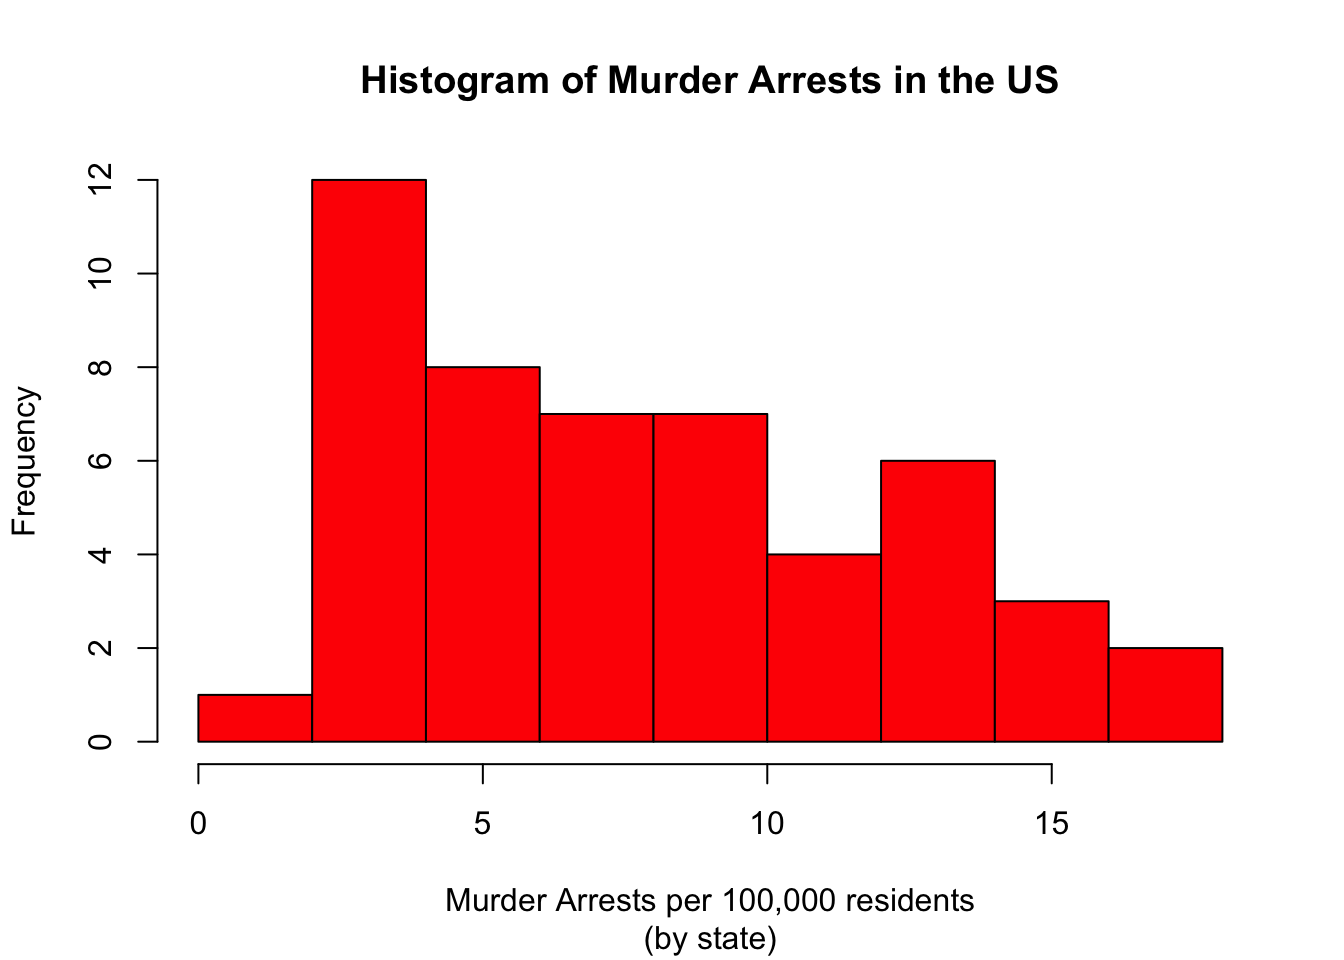
\includegraphics{Assignments_files/figure-latex/unnamed-chunk-6-1.pdf}

\hypertarget{problem-6}{%
\subsubsection{Problem 6}\label{problem-6}}

\emph{Please summarize \texttt{Murder} quantitatively. What are its mean
and median? What is the difference between mean and median? What is a
quartile, and why do you think R gives you the 1st Qu. and 3rd Qu.?}

\begin{Shaded}
\begin{Highlighting}[]
\FunctionTok{summary}\NormalTok{(dat}\SpecialCharTok{$}\NormalTok{Murder)}
\end{Highlighting}
\end{Shaded}

\begin{verbatim}
##    Min. 1st Qu.  Median    Mean 3rd Qu.    Max. 
##   0.800   4.075   7.250   7.788  11.250  17.400
\end{verbatim}

\textbf{Answer}: The mean of the Murder variable is 7.788 (murder
arrests per 100,000 residents of a state). The median is 7.250 (murder
arrests per 100,000 residents of a state). The difference between these
two values quantitatively is 0.538. The difference qualitatively is that
the mean represents the average number of murder arrests per 100,000
residents of all US states while the median is the middle value of the
data set, showing the data has a slight right skew. A quartile isdivides
the dataset into four parts, with Q1 being the median of the lower half
of the dataset and Q3 being the median of the upper half of the data
set. R gives you this information because quartiles can be helpful in
determining where a specific data point falls in the set; for example,
if a value for ``Murders'' is greater than Q3, 11.250, we can more
reasonably assume that this state has an exceptionally high murder rate
in comparison to other states in the US. If a state has a value for
``Murders'' that is less than 4.075, we can more reasonably assume that
this state is relatively safer than other US states!

\hypertarget{problem-7}{%
\subsubsection{Problem 7}\label{problem-7}}

\emph{Repeat the same steps you followed for \texttt{Murder}, for the
variables \texttt{Assault} and \texttt{Rape}. Now plot all three
histograms together. You can do this by using the command
\texttt{par(mfrow=c(3,1))} and then plotting each of the three. }

\begin{Shaded}
\begin{Highlighting}[]
\FunctionTok{hist}\NormalTok{(dat}\SpecialCharTok{$}\NormalTok{Assault, }\AttributeTok{col =} \StringTok{\textquotesingle{}red\textquotesingle{}}\NormalTok{, }\AttributeTok{ylab =} \StringTok{\textquotesingle{}Frequency\textquotesingle{}}\NormalTok{, }\AttributeTok{xlab =} \StringTok{\textquotesingle{}Assault Arrests per 100,000 residents\textquotesingle{}}\NormalTok{, }\AttributeTok{main =} \StringTok{\textquotesingle{}Histogram of Assault Arrests in the US\textquotesingle{}}\NormalTok{, }\AttributeTok{sub =} \StringTok{\textquotesingle{}(by state)\textquotesingle{}}\NormalTok{)}
\end{Highlighting}
\end{Shaded}

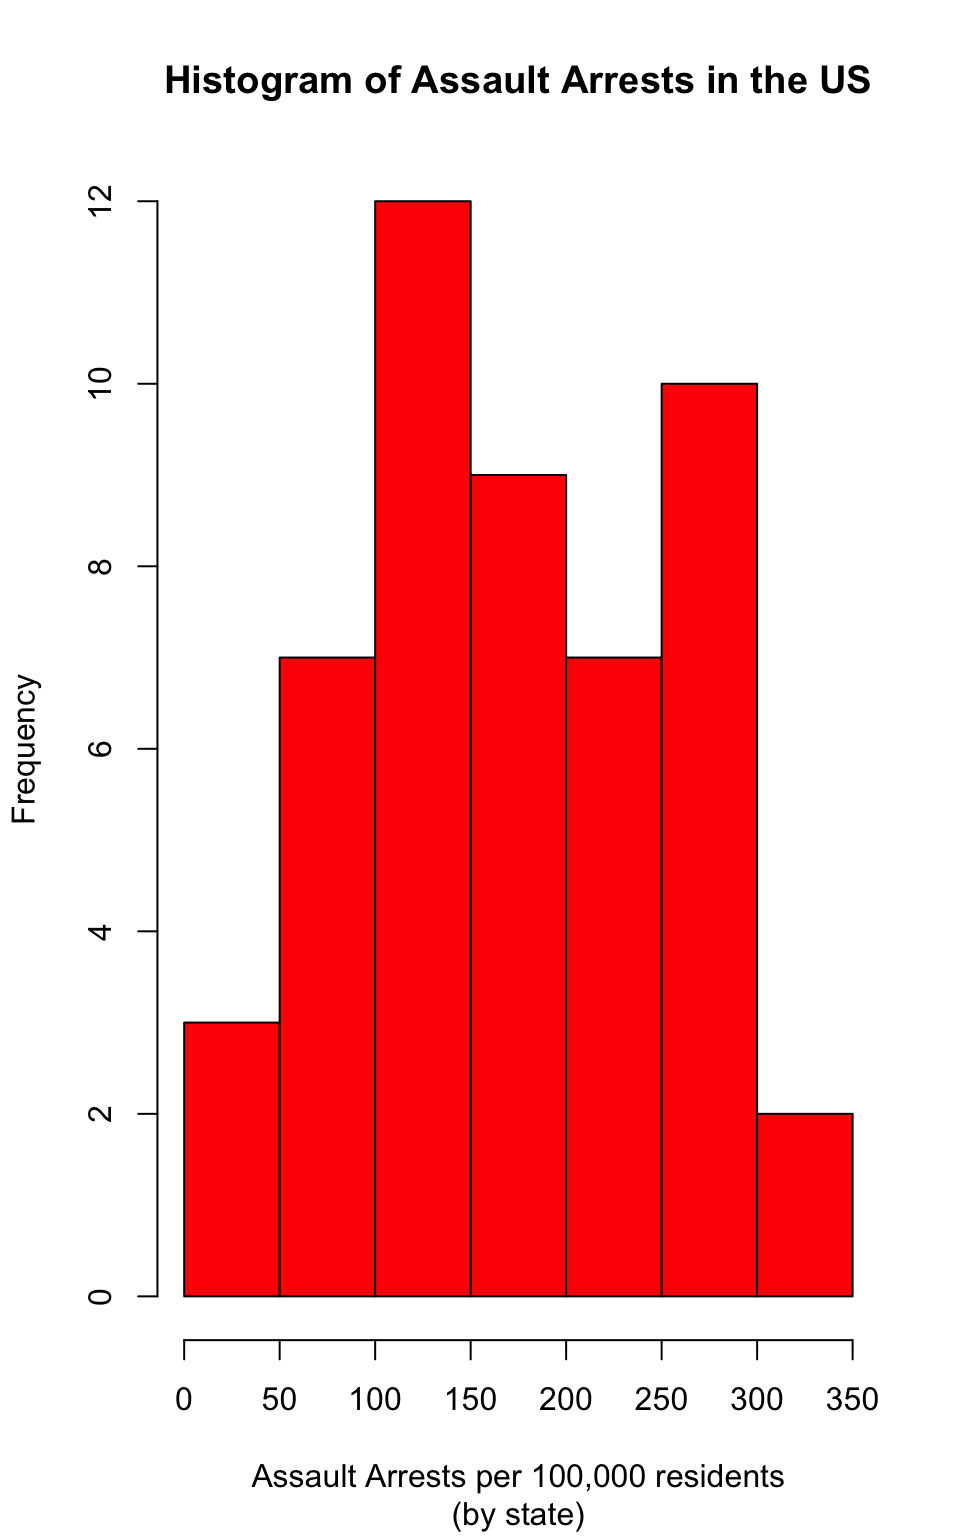
\includegraphics{Assignments_files/figure-latex/unnamed-chunk-8-1.pdf}

\begin{Shaded}
\begin{Highlighting}[]
\FunctionTok{summary}\NormalTok{(dat}\SpecialCharTok{$}\NormalTok{Assault)}
\end{Highlighting}
\end{Shaded}

\begin{verbatim}
##    Min. 1st Qu.  Median    Mean 3rd Qu.    Max. 
##    45.0   109.0   159.0   170.8   249.0   337.0
\end{verbatim}

\begin{Shaded}
\begin{Highlighting}[]
\FunctionTok{hist}\NormalTok{(dat}\SpecialCharTok{$}\NormalTok{Rape, }\AttributeTok{col =} \StringTok{\textquotesingle{}red\textquotesingle{}}\NormalTok{, }\AttributeTok{ylab =} \StringTok{\textquotesingle{}Frequency\textquotesingle{}}\NormalTok{, }\AttributeTok{xlab =} \StringTok{\textquotesingle{}Rape Arrests per 100,000 residents\textquotesingle{}}\NormalTok{, }\AttributeTok{main =} \StringTok{\textquotesingle{}Histogram of Rape Arrests in the US\textquotesingle{}}\NormalTok{, }\AttributeTok{sub =} \StringTok{\textquotesingle{}(by state)\textquotesingle{}}\NormalTok{)}
\end{Highlighting}
\end{Shaded}

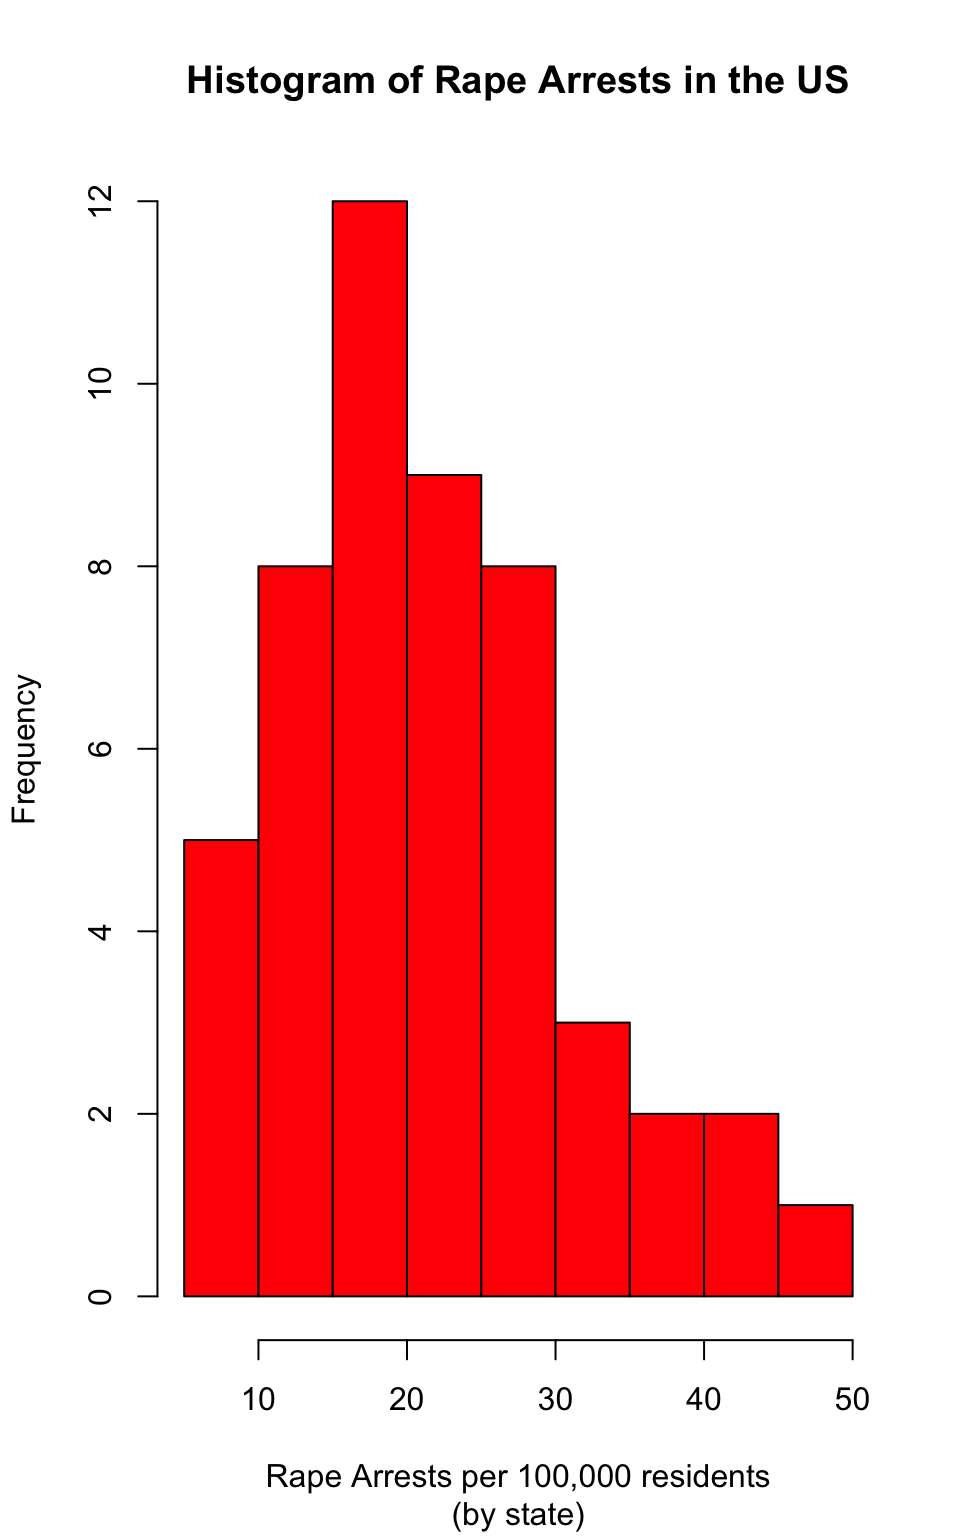
\includegraphics{Assignments_files/figure-latex/unnamed-chunk-8-2.pdf}

\begin{Shaded}
\begin{Highlighting}[]
\FunctionTok{summary}\NormalTok{(dat}\SpecialCharTok{$}\NormalTok{Rape)}
\end{Highlighting}
\end{Shaded}

\begin{verbatim}
##    Min. 1st Qu.  Median    Mean 3rd Qu.    Max. 
##    7.30   15.07   20.10   21.23   26.18   46.00
\end{verbatim}

\begin{Shaded}
\begin{Highlighting}[]
\FunctionTok{par}\NormalTok{(}\AttributeTok{mfrow=}\FunctionTok{c}\NormalTok{(}\DecValTok{3}\NormalTok{,}\DecValTok{1}\NormalTok{))}
\FunctionTok{hist}\NormalTok{(dat}\SpecialCharTok{$}\NormalTok{Murder, }\AttributeTok{col =} \StringTok{\textquotesingle{}red\textquotesingle{}}\NormalTok{, }\AttributeTok{ylab =} \StringTok{\textquotesingle{}Frequency\textquotesingle{}}\NormalTok{, }\AttributeTok{xlab =} \StringTok{\textquotesingle{}Murder Arrests per 100,000 residents\textquotesingle{}}\NormalTok{, }\AttributeTok{main =} \StringTok{\textquotesingle{}Histogram of Murder Arrests in the US\textquotesingle{}}\NormalTok{, }\AttributeTok{sub =} \StringTok{\textquotesingle{}(by state)\textquotesingle{}}\NormalTok{)}
\FunctionTok{hist}\NormalTok{(dat}\SpecialCharTok{$}\NormalTok{Assault, }\AttributeTok{col =} \StringTok{\textquotesingle{}red\textquotesingle{}}\NormalTok{, }\AttributeTok{ylab =} \StringTok{\textquotesingle{}Frequency\textquotesingle{}}\NormalTok{, }\AttributeTok{xlab =} \StringTok{\textquotesingle{}Assault Arrests per 100,000 residents\textquotesingle{}}\NormalTok{, }\AttributeTok{main =} \StringTok{\textquotesingle{}Histogram of Assault Arrests in the US\textquotesingle{}}\NormalTok{, }\AttributeTok{sub =} \StringTok{\textquotesingle{}(by state)\textquotesingle{}}\NormalTok{)}
\FunctionTok{summary}\NormalTok{(dat}\SpecialCharTok{$}\NormalTok{Assault)}
\end{Highlighting}
\end{Shaded}

\begin{verbatim}
##    Min. 1st Qu.  Median    Mean 3rd Qu.    Max. 
##    45.0   109.0   159.0   170.8   249.0   337.0
\end{verbatim}

\begin{Shaded}
\begin{Highlighting}[]
\FunctionTok{hist}\NormalTok{(dat}\SpecialCharTok{$}\NormalTok{Rape, }\AttributeTok{col =} \StringTok{\textquotesingle{}red\textquotesingle{}}\NormalTok{, }\AttributeTok{ylab =} \StringTok{\textquotesingle{}Frequency\textquotesingle{}}\NormalTok{, }\AttributeTok{xlab =} \StringTok{\textquotesingle{}Rape Arrests per 100,000 residents\textquotesingle{}}\NormalTok{, }\AttributeTok{main =} \StringTok{\textquotesingle{}Histogram of Rape Arrests in the US\textquotesingle{}}\NormalTok{, }\AttributeTok{sub =} \StringTok{\textquotesingle{}(by state)\textquotesingle{}}\NormalTok{)}
\end{Highlighting}
\end{Shaded}

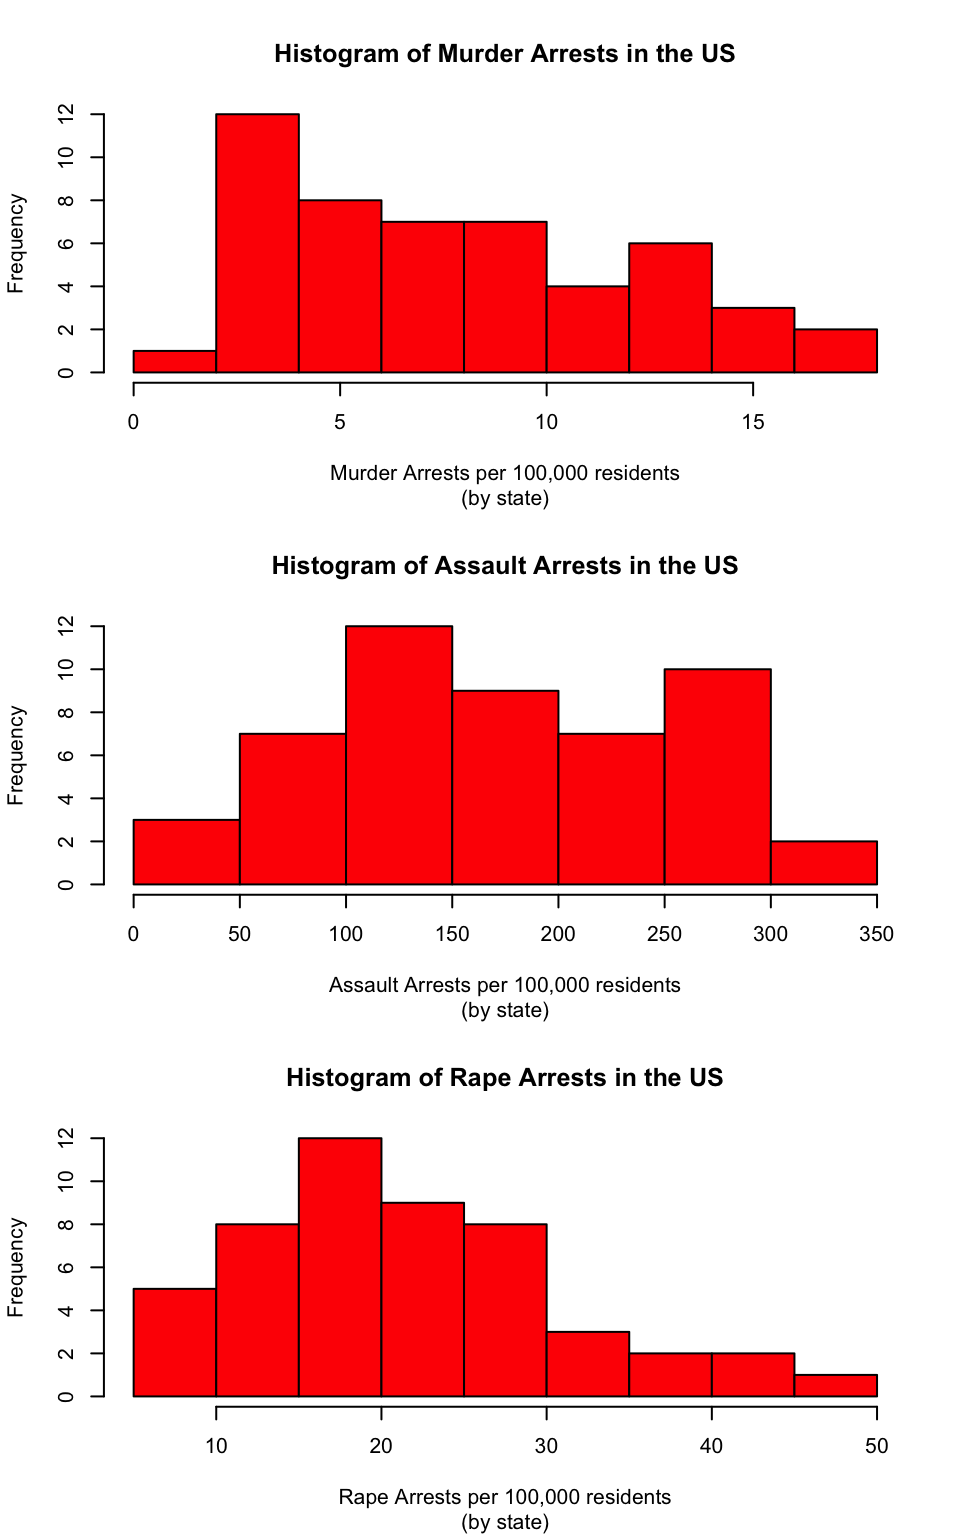
\includegraphics{Assignments_files/figure-latex/unnamed-chunk-8-3.pdf}

\emph{What does the command par do, in your own words (you can look this
up by asking R \texttt{?par})?}

\textbf{Answer}: The par function allows an R user to look at the
graphical parameters that control how graphs are displayed. In the case
of the par(mfrow=c(3,1)) function, we are able to not only look at the
graphical parameters, but control them so that we can decide how many
subplots we want displayed.

\emph{What can you learn from plotting the histograms together?}

\textbf{Answer}: From plotting the histograms together, we can view a
comparison of the distributions in relation to each other, examining
skew and quartile arrangement to see how distributions vary by crime
type. On a more general note, plotting the histograms together allows us
to see generally how frequency and distribution relationships among
multiple variables interact, allowing a viewer a more clear image of the
relationship between variables while still being able to view a more
individualistic look at each histogram.

\hypertarget{problem-8}{%
\subsubsection{Problem 8}\label{problem-8}}

\emph{In the console below (not in text), type
\texttt{install.packages("maps")} and press Enter, and then type
\texttt{install.packages("ggplot2")} and press Enter. This will install
the packages so you can load the libraries.}

\emph{Run this code:}

\begin{Shaded}
\begin{Highlighting}[]
\FunctionTok{library}\NormalTok{(maps) }
\FunctionTok{library}\NormalTok{(ggplot2) }

\FunctionTok{ggplot}\NormalTok{(dat, }\FunctionTok{aes}\NormalTok{(}\AttributeTok{map\_id=}\NormalTok{state, }\AttributeTok{fill=}\NormalTok{Murder)) }\SpecialCharTok{+} 
  \FunctionTok{geom\_map}\NormalTok{(}\AttributeTok{map=}\FunctionTok{map\_data}\NormalTok{(}\StringTok{"state"}\NormalTok{)) }\SpecialCharTok{+} 
  \FunctionTok{expand\_limits}\NormalTok{(}\AttributeTok{x=}\FunctionTok{map\_data}\NormalTok{(}\StringTok{"state"}\NormalTok{)}\SpecialCharTok{$}\NormalTok{long, }\AttributeTok{y=}\FunctionTok{map\_data}\NormalTok{(}\StringTok{"state"}\NormalTok{)}\SpecialCharTok{$}\NormalTok{lat)}
\end{Highlighting}
\end{Shaded}

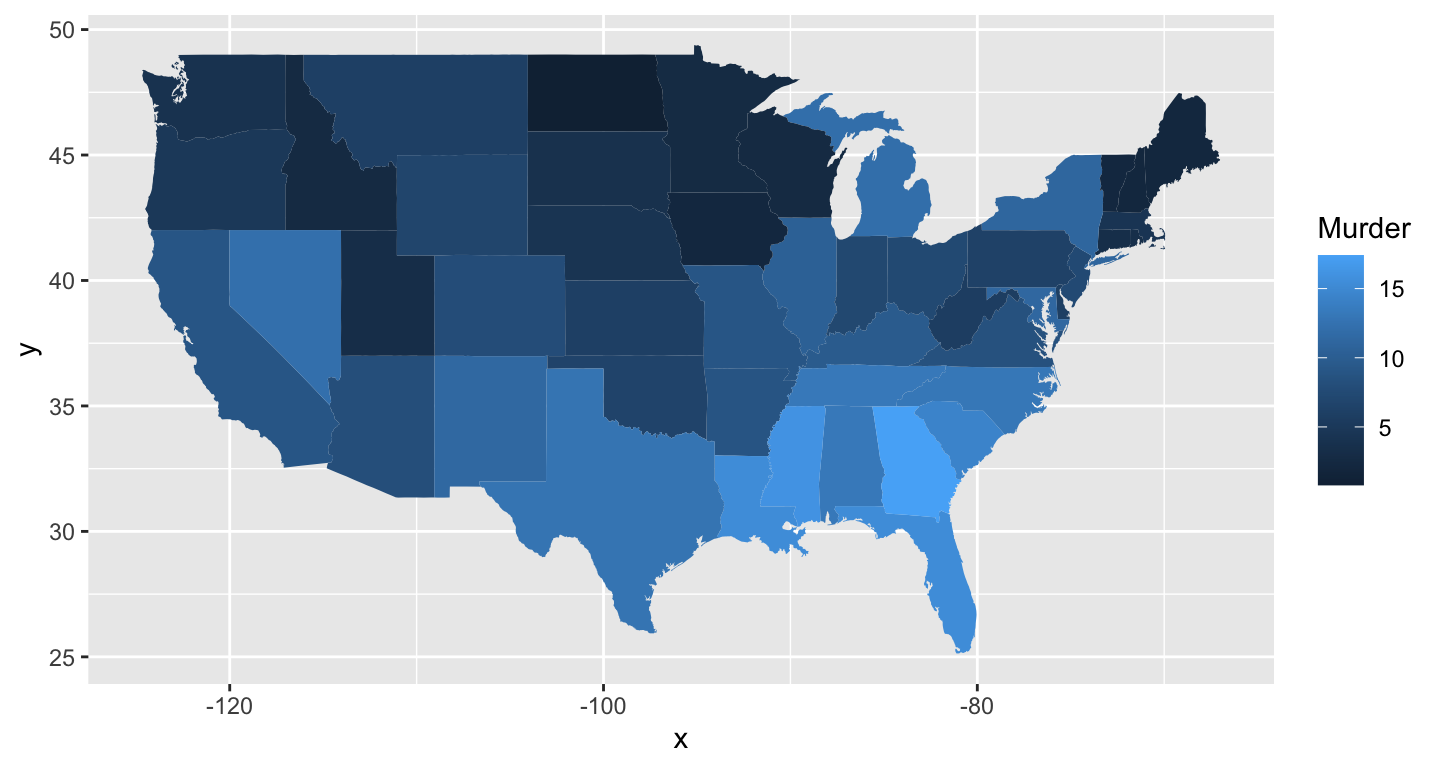
\includegraphics{Assignments_files/figure-latex/unnamed-chunk-9-1.pdf}

What does this code do? Explain what each line is doing.

\textbf{Answer}: ggplot is the most basic implementation of any data
visualization in R. In this instance, the first line of code is filling
out the basic information of the data visual by specifying the variables
which are involved in the plot. The second line of code employs the maps
package and ggplot2 package to choose specifically to create a mapping
of the selected variables, using states as the selected implementation
of the map. The third line employs the expand\_limit function in order
to ensure that the limits of the visualization include a single value
for all aspects of the plot, implying what should be included in the
scale.

\[\\[2in]\]

\end{document}
